\section{Appendix}

\setlength{\unitlength}{0.8cm}
  \begin{figure}[H]
  \centering
  \begin{minipage}[!hp]{0.45\linewidth}
  \centering
    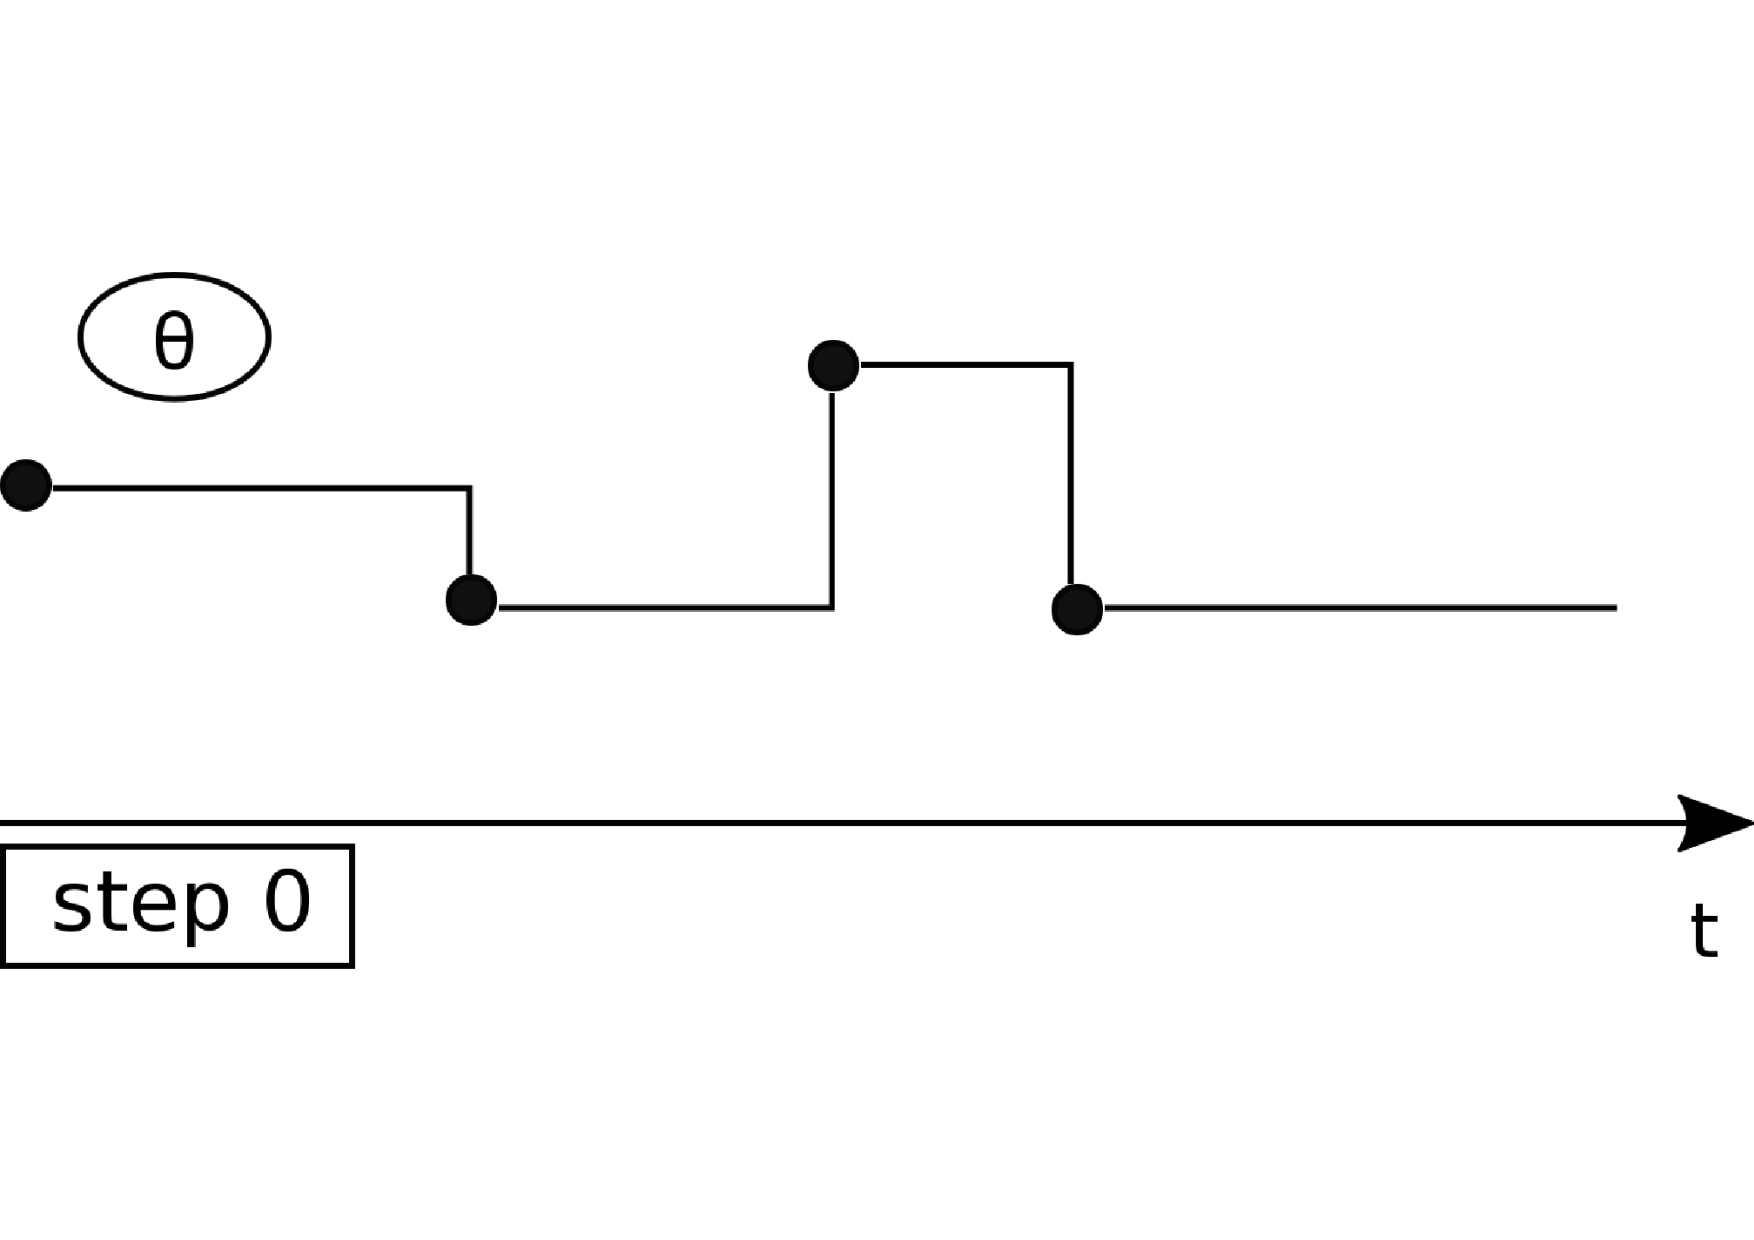
\includegraphics [width=0.70\textwidth, angle=0]{figs/plotn0.pdf}
      \end{minipage}
  \begin{minipage}[!hp]{0.45\linewidth}
  \centering
    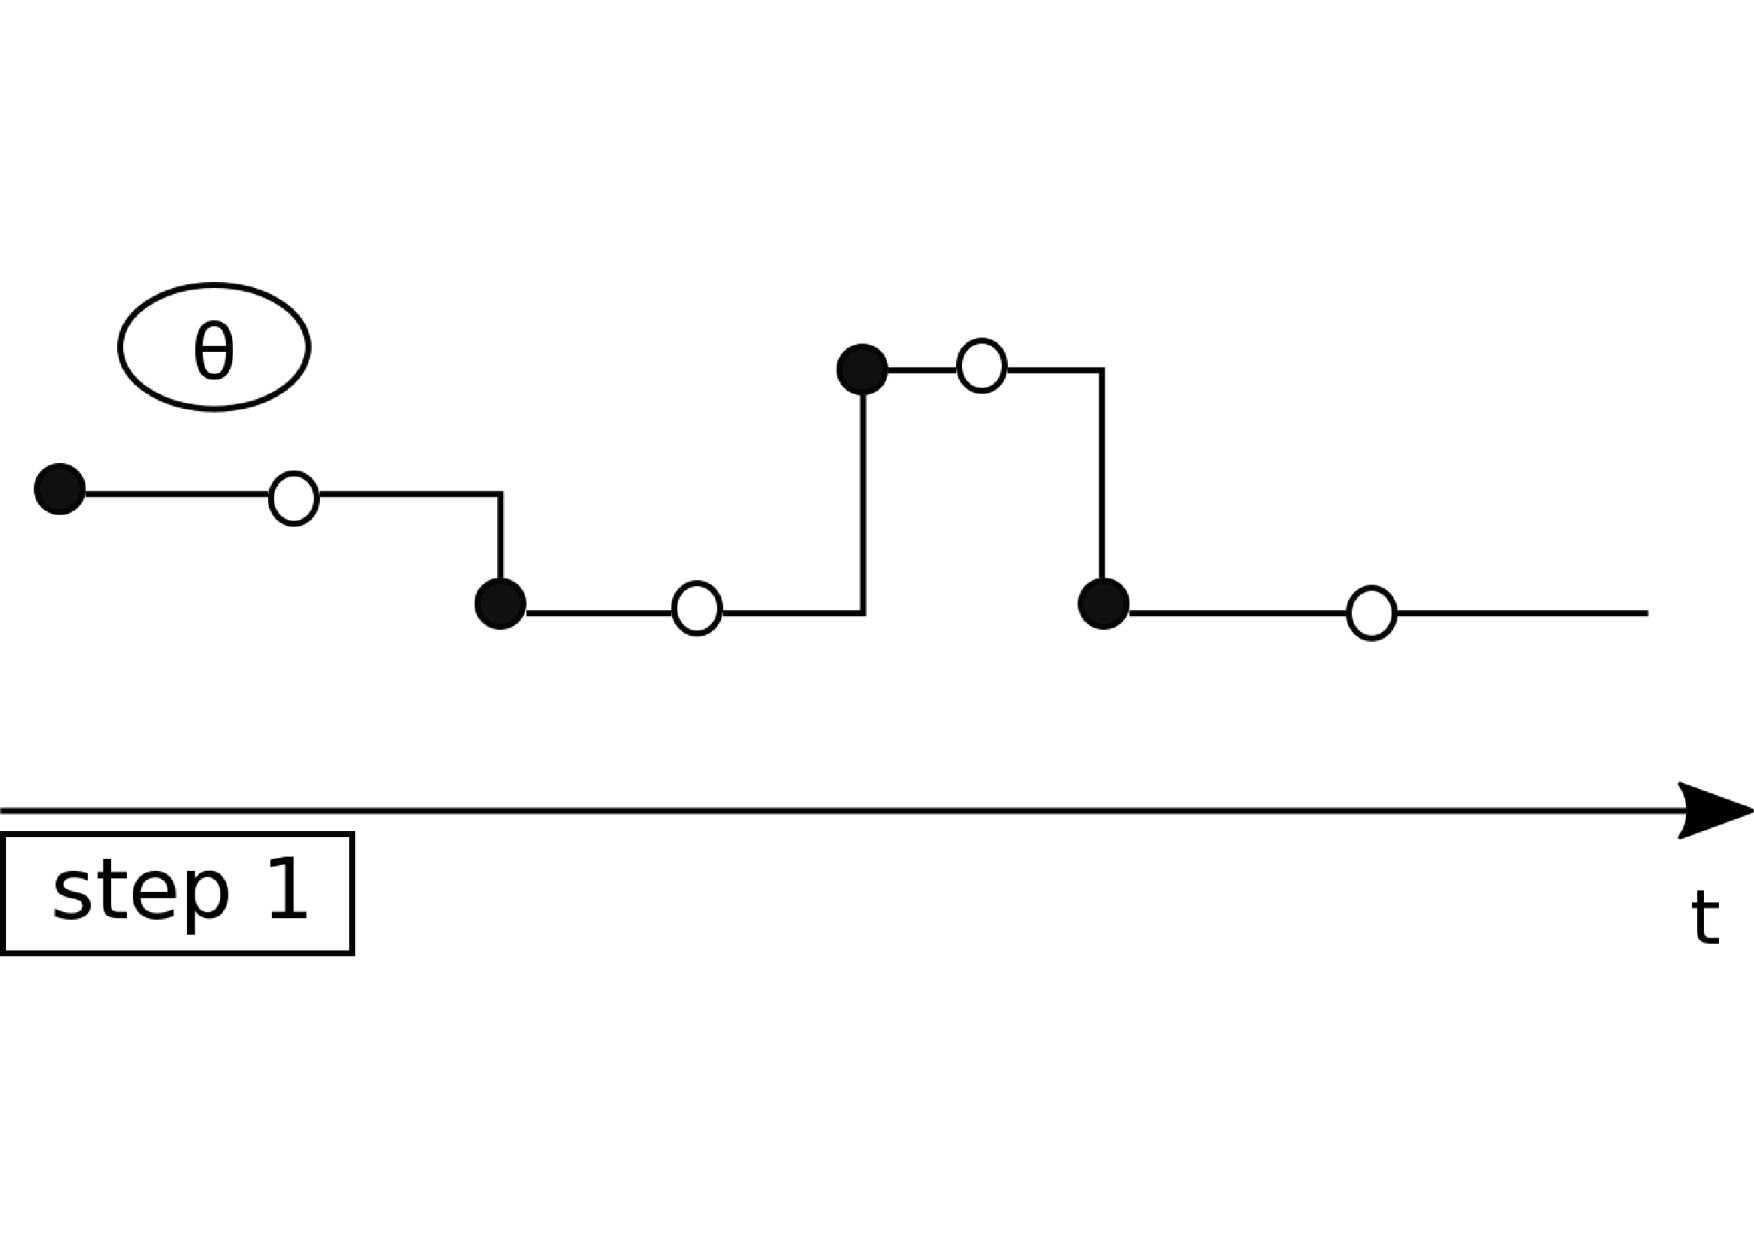
\includegraphics [width=0.70\textwidth, angle=0]{figs/plotn1.pdf}
    \vspace{-0 in}
  \end{minipage}
  \begin{minipage}[!hp]{0.45\linewidth}
  \centering
    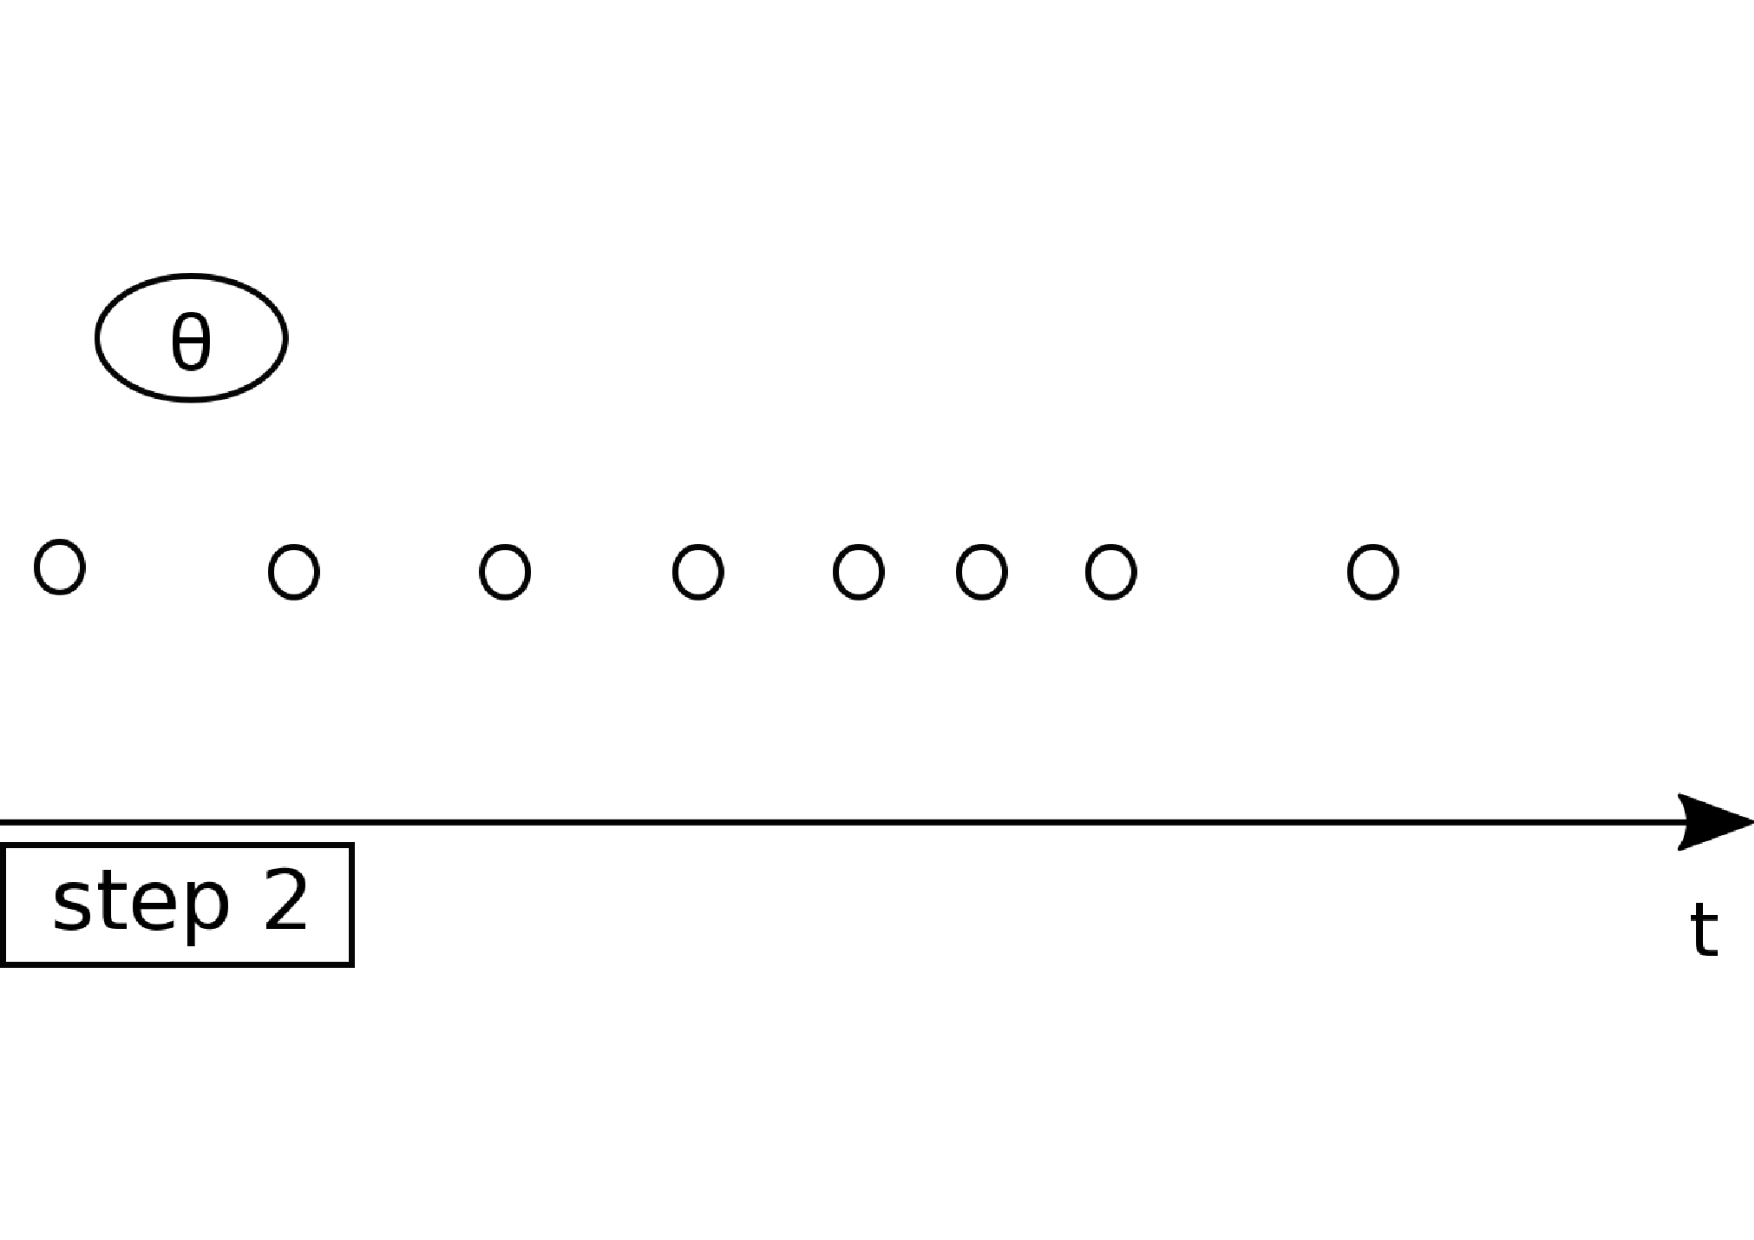
\includegraphics [width=0.70\textwidth, angle=0]{figs/plotn2.pdf}
    \vspace{-0 in}
  \end{minipage}
  \begin{minipage}[!hp]{0.45\linewidth}
  \centering
    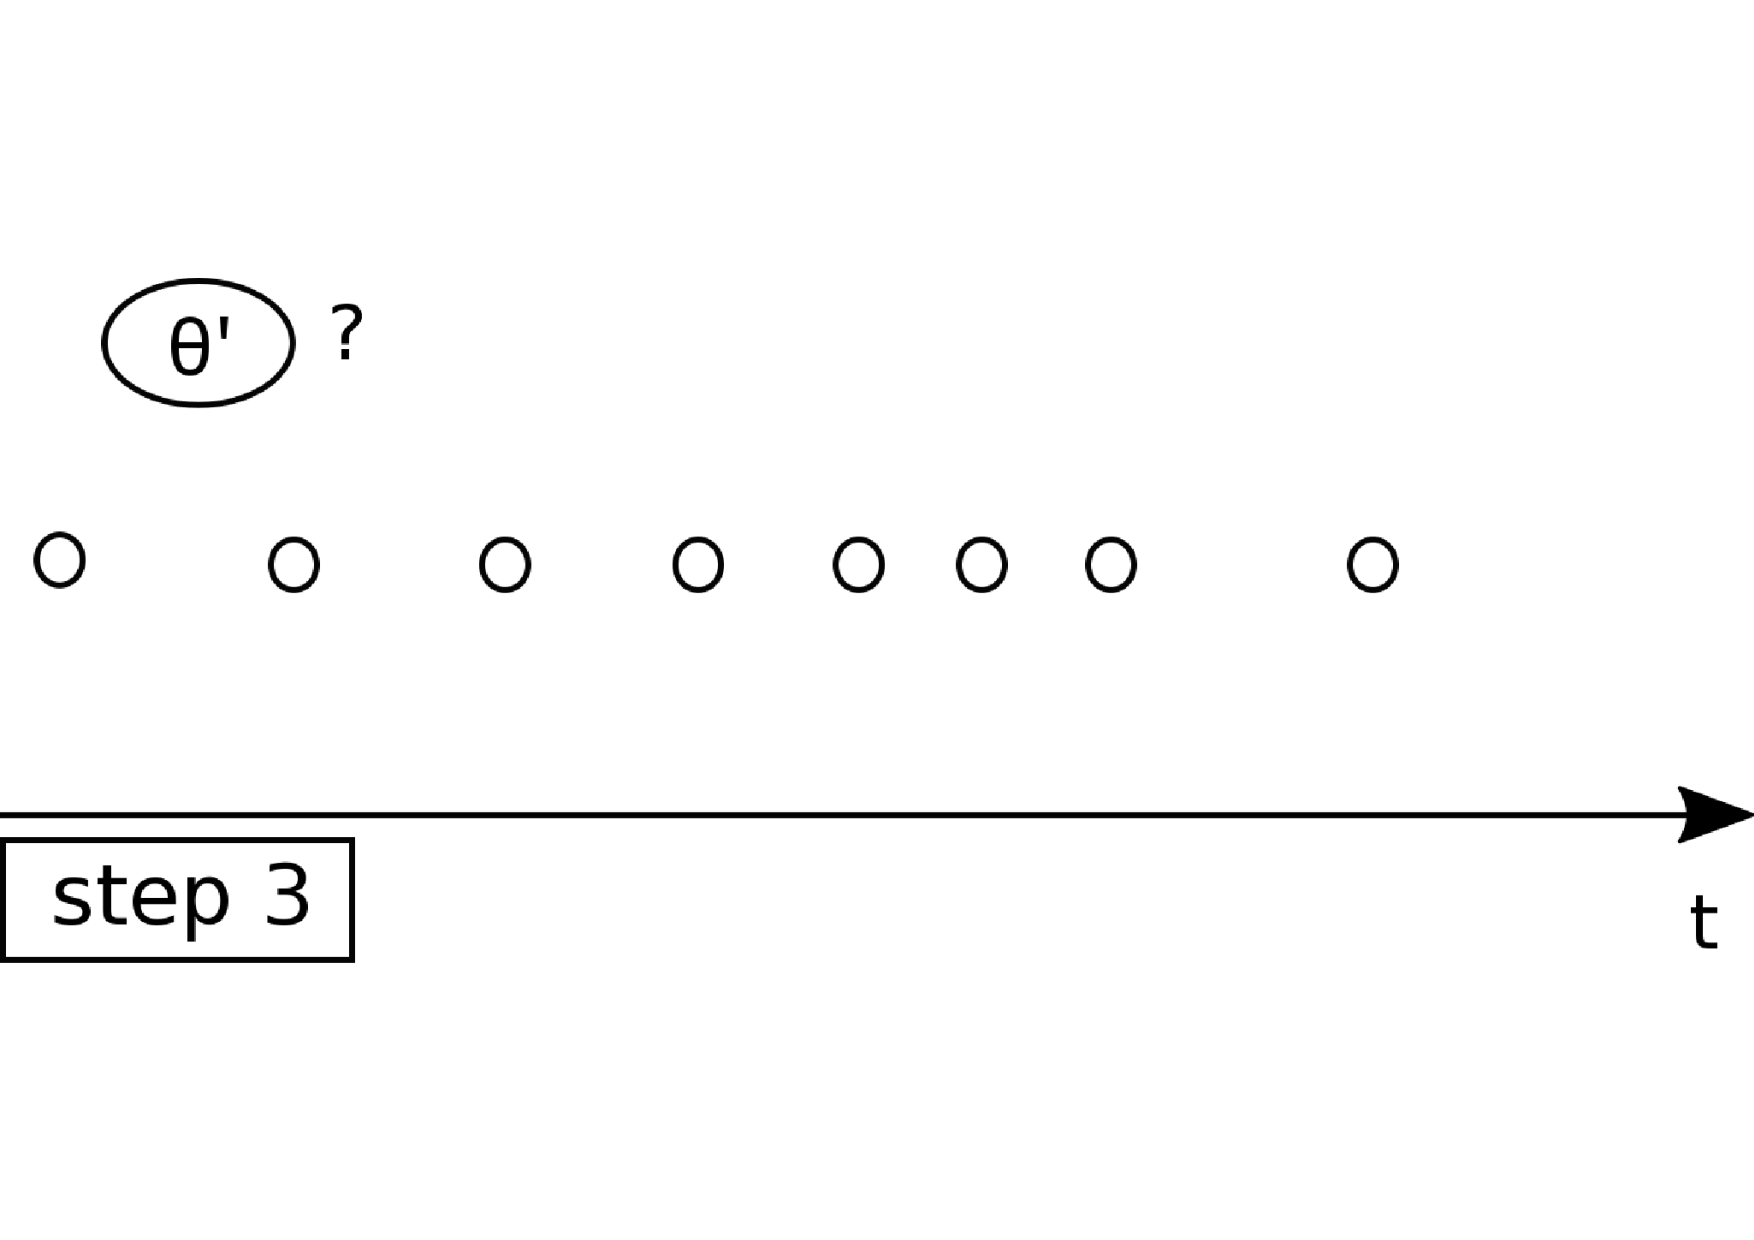
\includegraphics [width=0.70\textwidth, angle=0]{figs/plotn3.pdf}
    \vspace{-0 in}
  \end{minipage}
  \begin{minipage}[!hp]{0.45\linewidth}
  \centering
    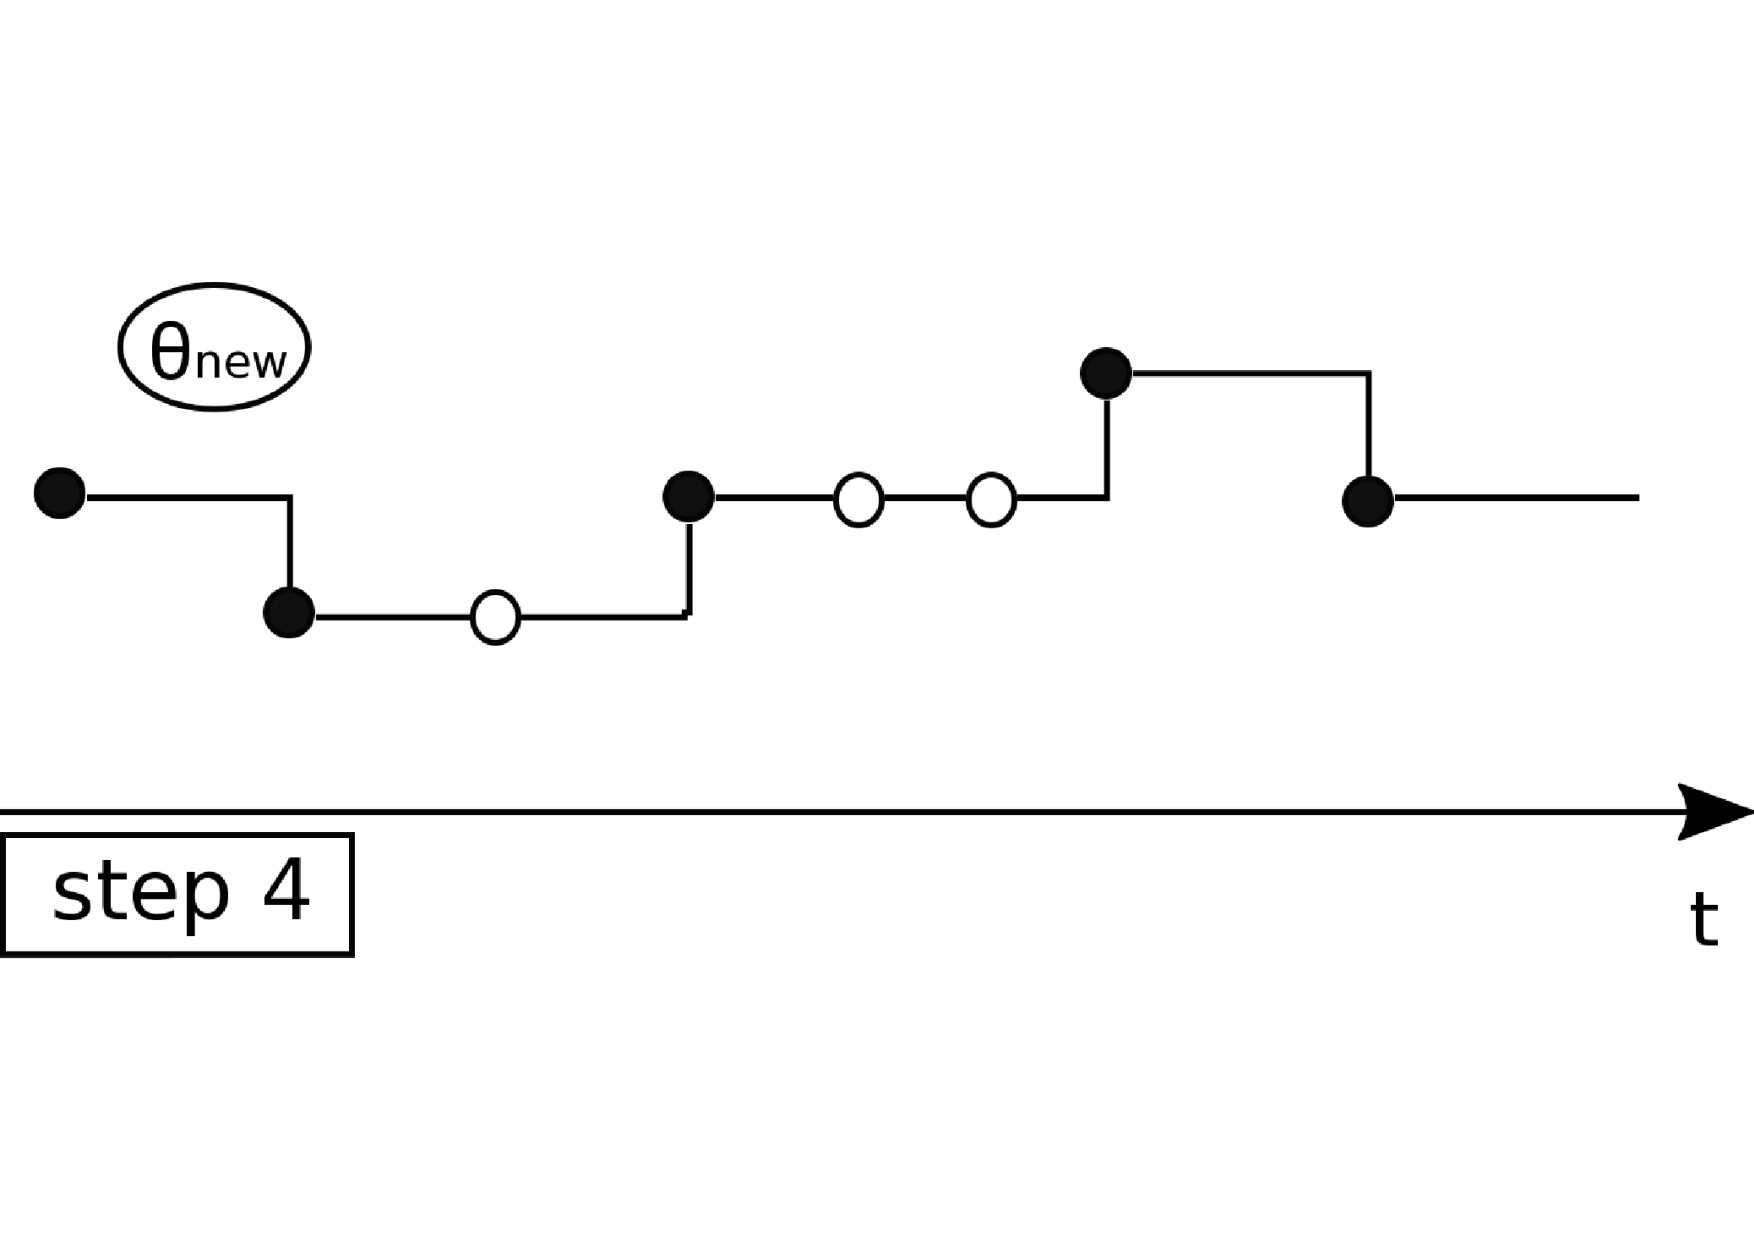
\includegraphics [width=0.70\textwidth, angle=0]{figs/plotn4.pdf}
    \vspace{-0 in}
  \end{minipage}
  \begin{minipage}[!hp]{0.45\linewidth}
  \centering
    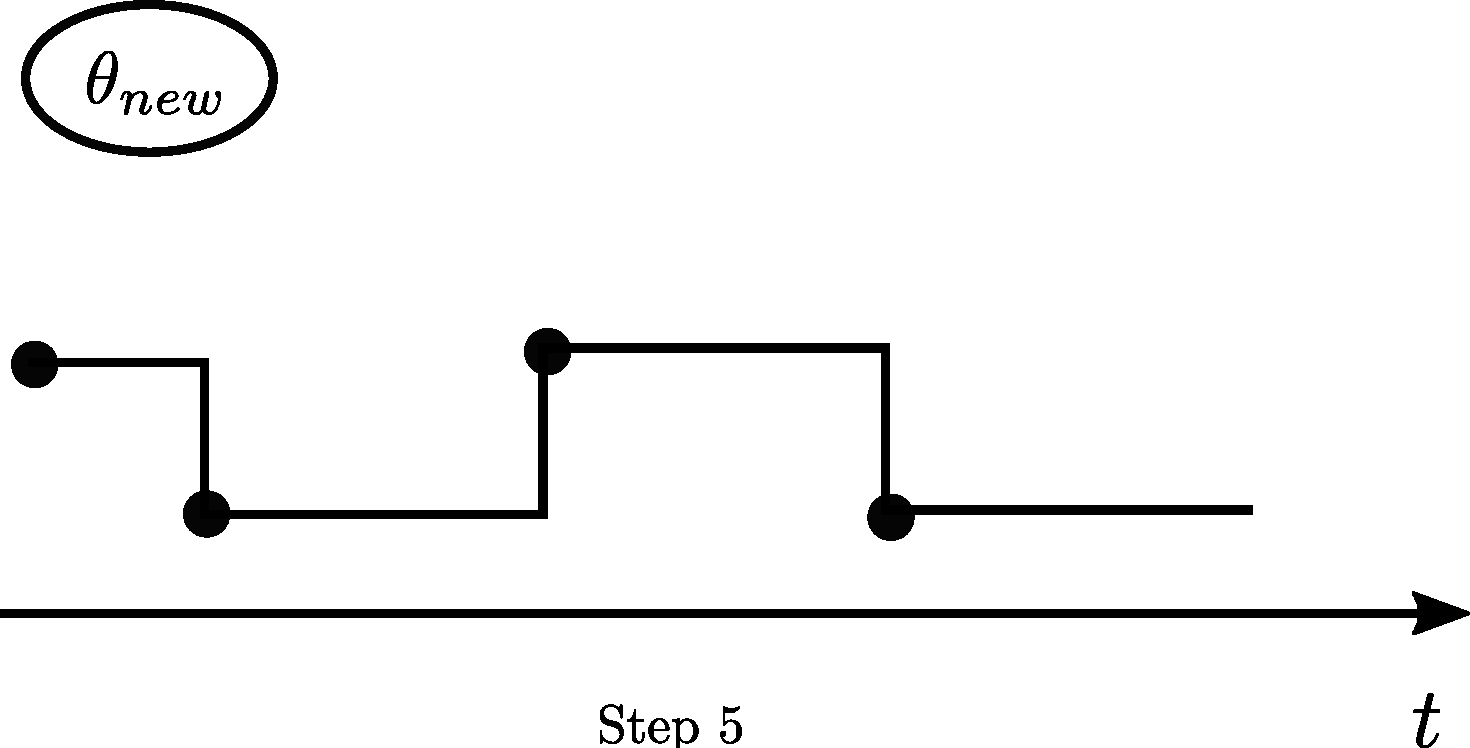
\includegraphics [width=0.70\textwidth, angle=0]{figs/plotn5.pdf}
    \vspace{-0 in}
  \end{minipage}
  \caption{\Naive\ MH-algorithm. Step 0 to 2: sample thinned events
  and discard state information to get a random grid. Step 3: 
propose a new parameter $\theta'$, and accept or reject by making
a forward pass on the grid. Steps 4 to 5: make a backward pass using
the accepted parameter and discard self-transitions to produce a new
trajectory.}
   \label{fig:naive_mh}

  \end{figure}

\setlength{\unitlength}{0.8cm}
  \begin{figure}[H]
  \centering
  \begin{minipage}[!hp]{0.45\linewidth}
  \centering
    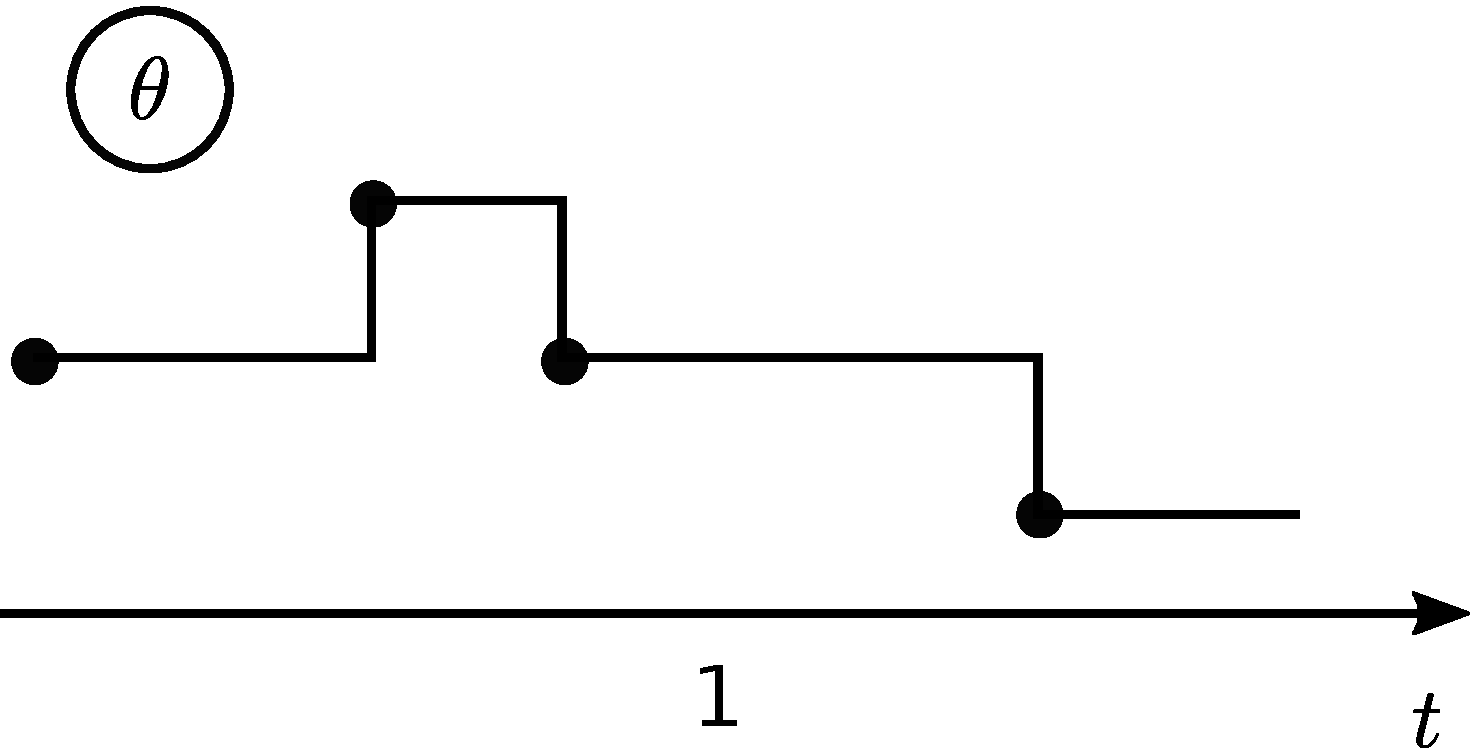
\includegraphics [width=0.70\textwidth, angle=0]{figs/plot0.pdf}
      \end{minipage}
  \begin{minipage}[hp]{0.45\linewidth}
  \centering
    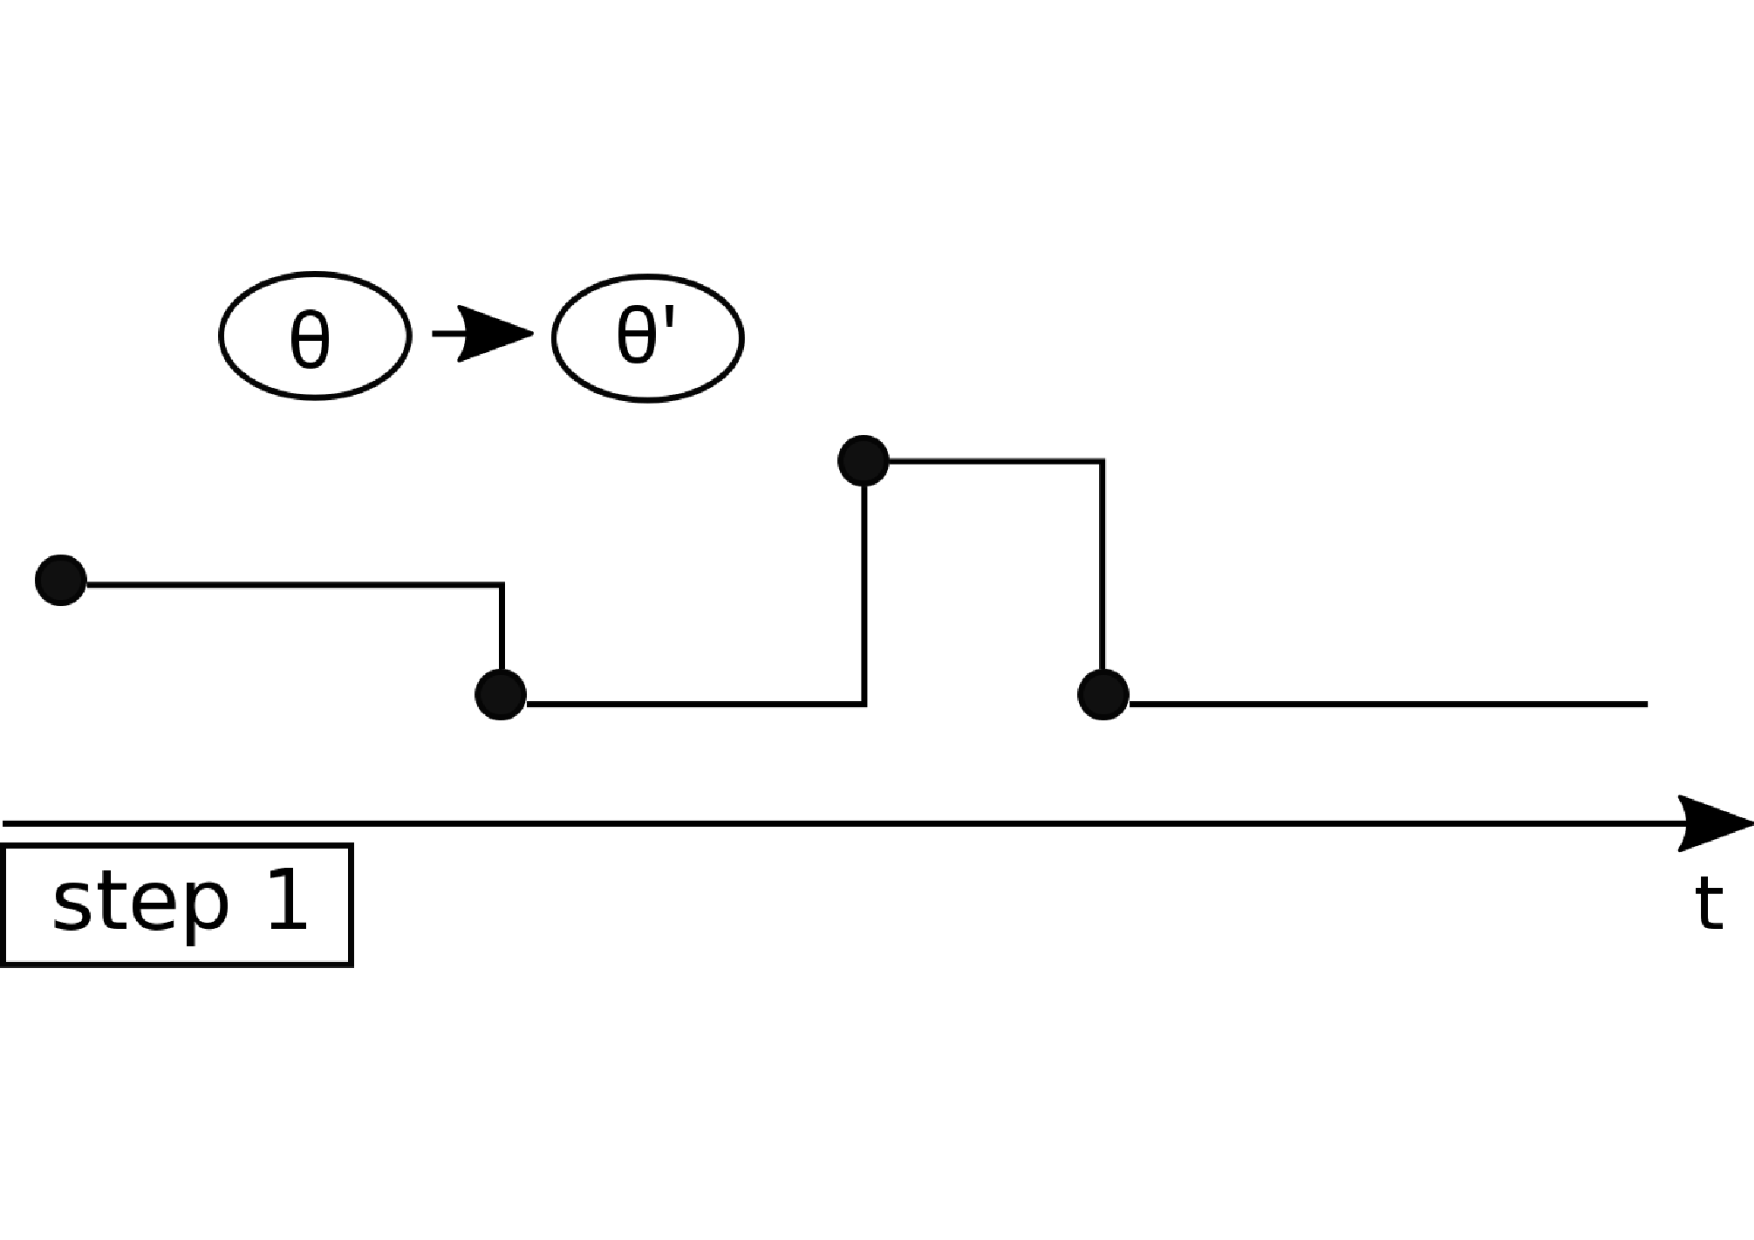
\includegraphics [width=0.70\textwidth, angle=0]{figs/plot1.pdf}
    \vspace{-0 in}
  \end{minipage}
  \begin{minipage}[hp]{0.45\linewidth}
  \centering
    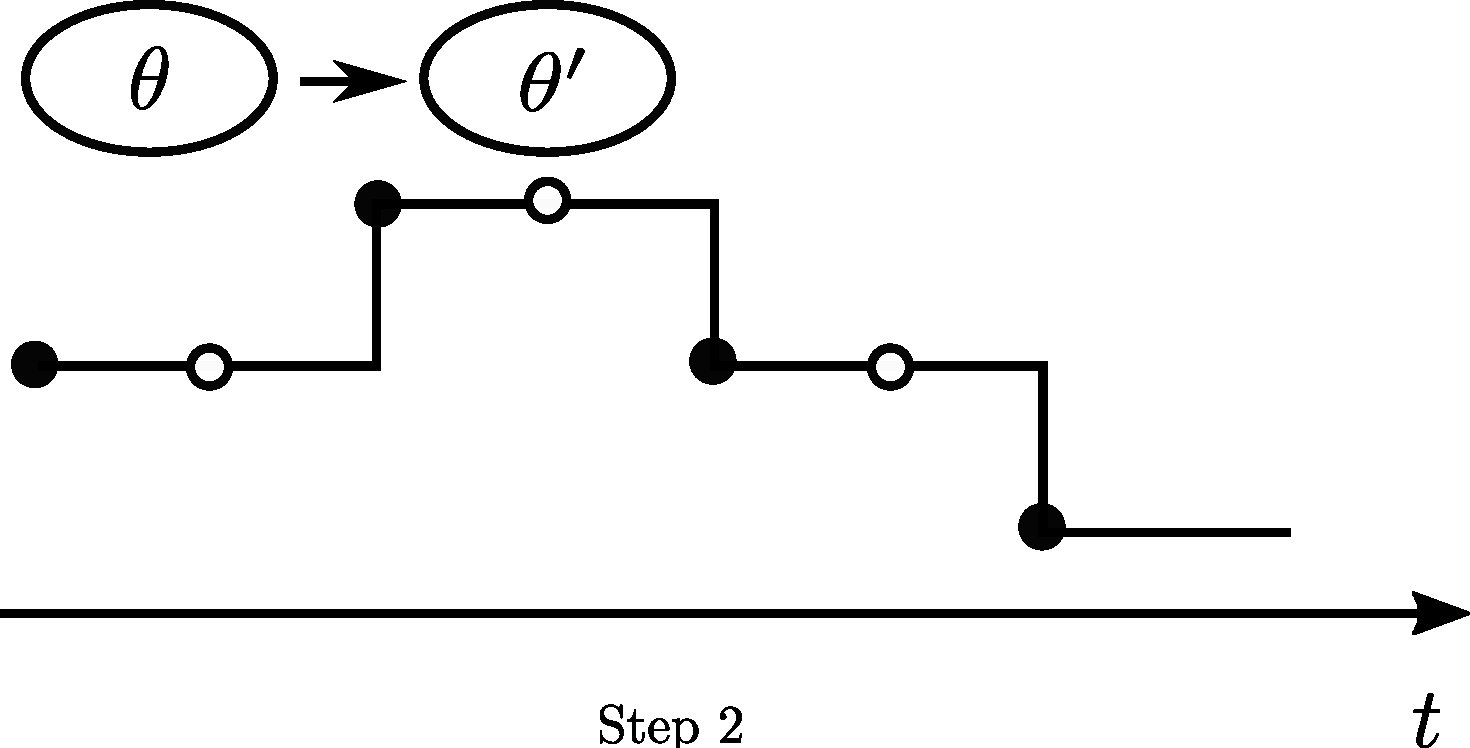
\includegraphics [width=0.70\textwidth, angle=0]{figs/plot2.pdf}
    \vspace{-0 in}
  \end{minipage}
  \begin{minipage}[hp]{0.45\linewidth}
  \centering
    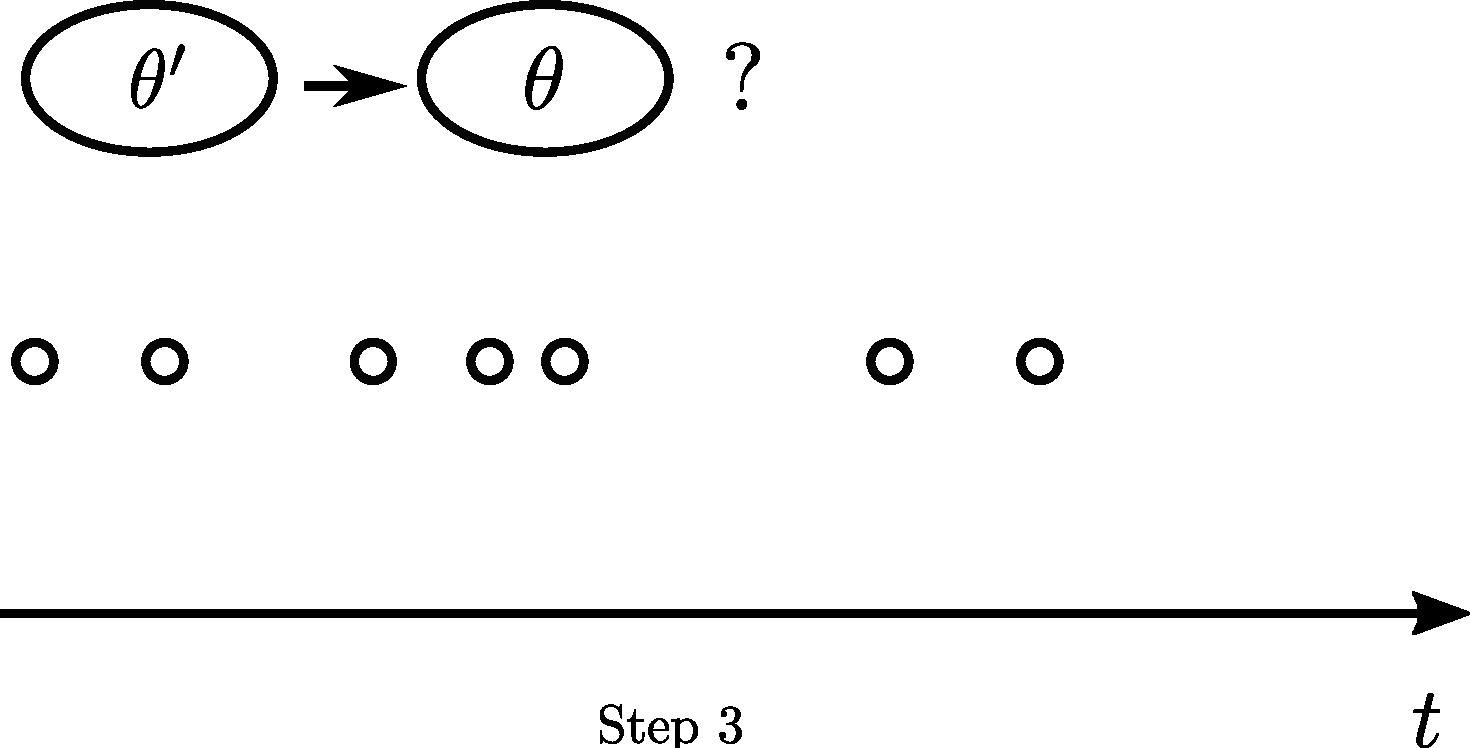
\includegraphics [width=0.70\textwidth, angle=0]{figs/plot3.pdf}
    \vspace{-0 in}
  \end{minipage}
% \begin{minipage}[hp]{0.45\linewidth}
% \centering
%   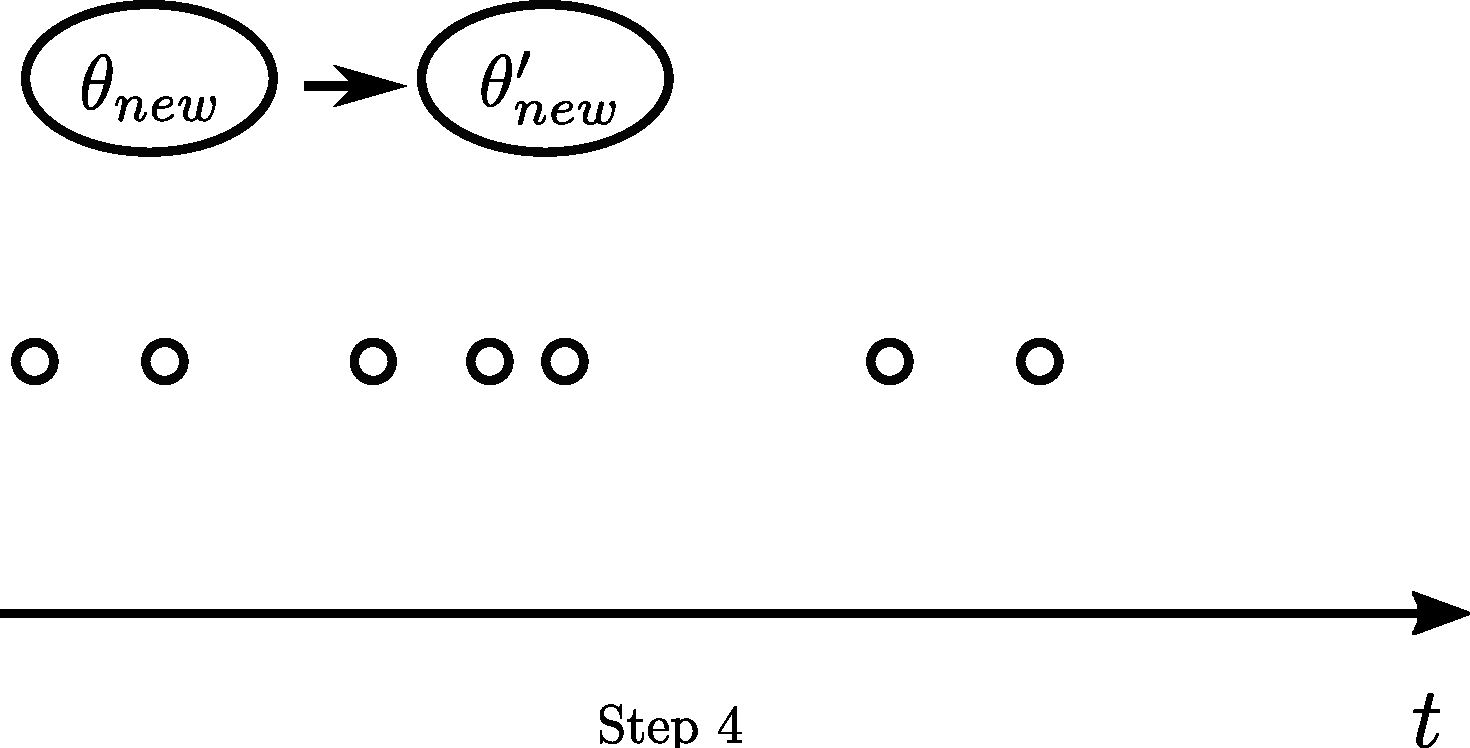
\includegraphics [width=0.70\textwidth, angle=0]{figs/plot4.pdf}
%   \vspace{-0 in}
% \end{minipage}
  \begin{minipage}[hp]{0.45\linewidth}
  \centering
    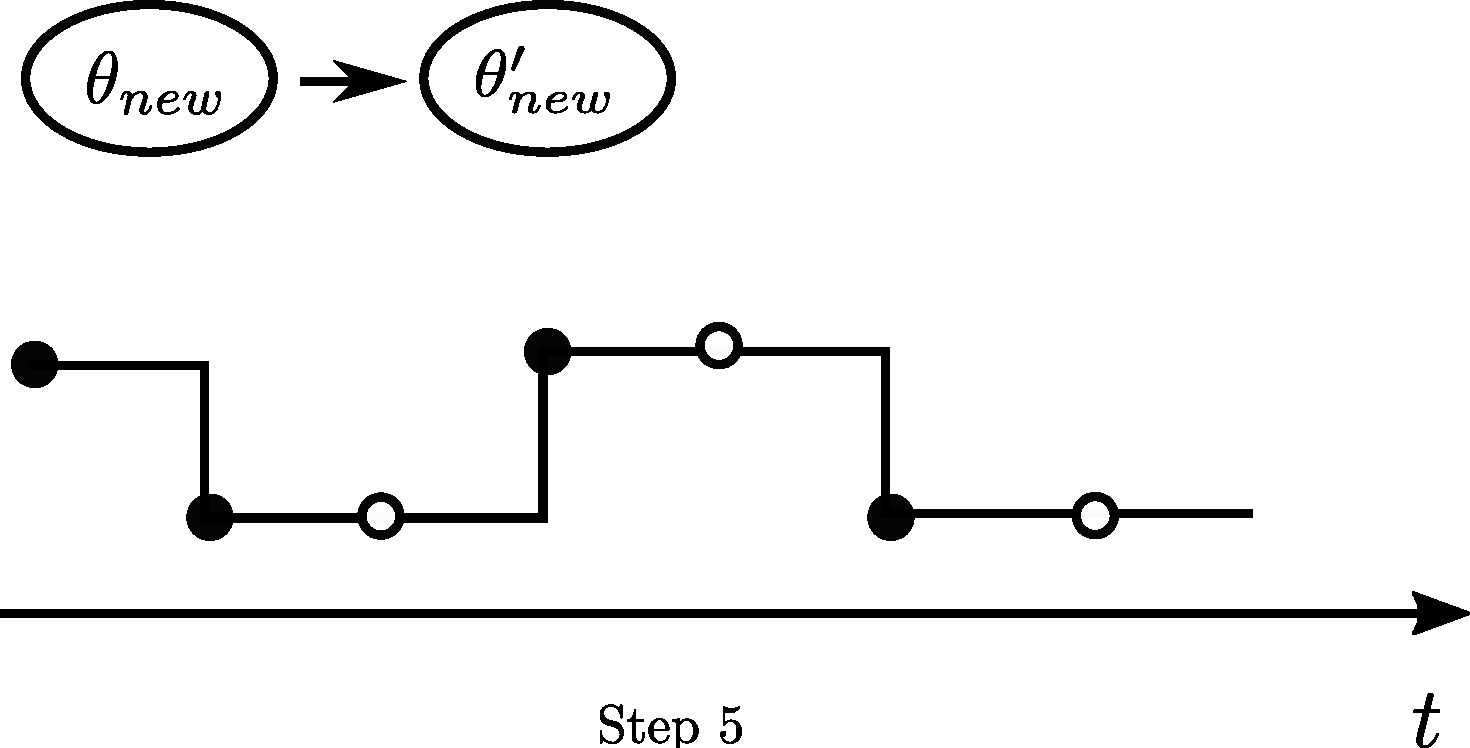
\includegraphics [width=0.70\textwidth, angle=0]{figs/plot5.pdf}
    \vspace{-0 in}
  \end{minipage}
  \begin{minipage}[hp]{0.45\linewidth}
  \centering
    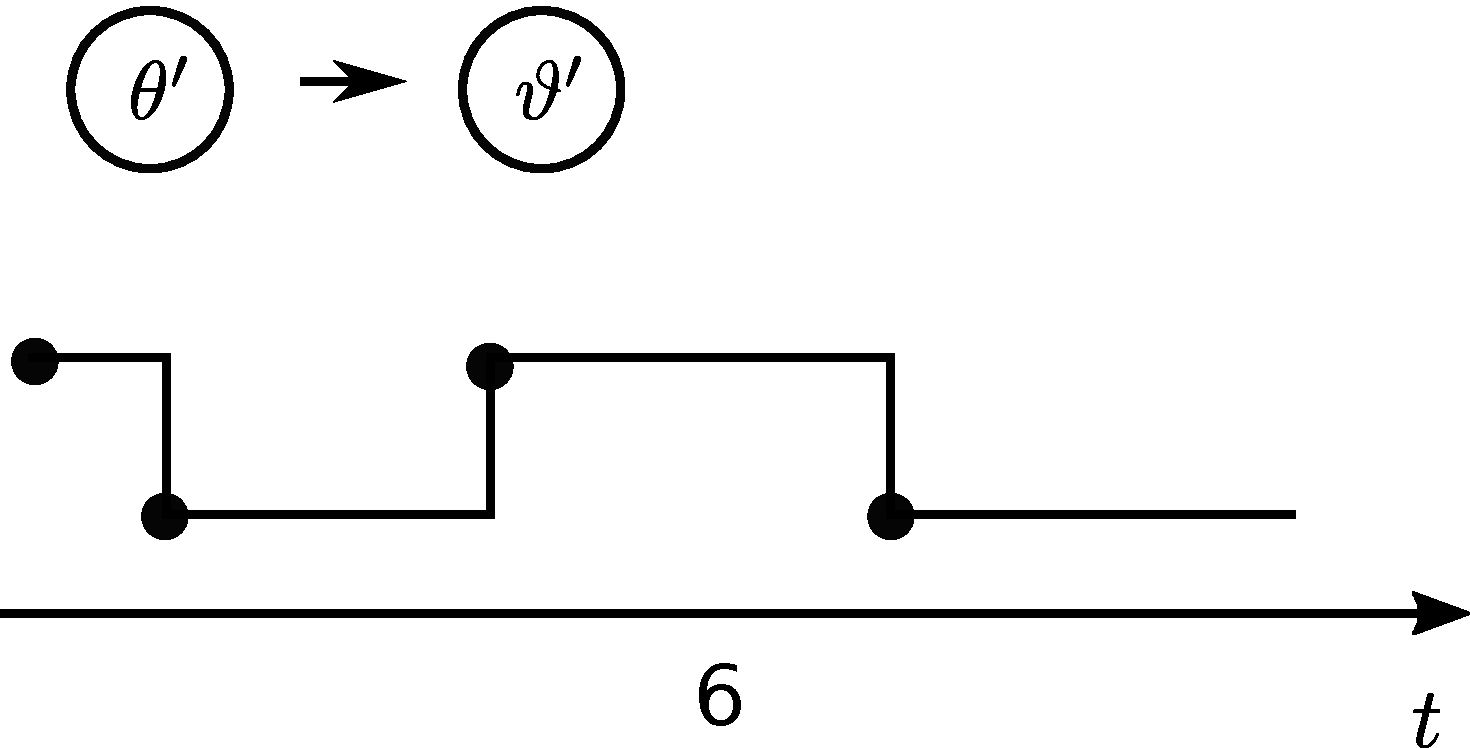
\includegraphics [width=0.70\textwidth, angle=0]{figs/plot6.pdf}
    \vspace{-0 in}
  \end{minipage}
    \caption{Steps 0-3: Starting with a trajectory and parameter $\theta$,
      simulate an auxiliary parameter $\theta^*$, and then the thinned events
      $U$ from a rate $\Omega(\theta) + \Omega(\theta^*) - A_{S(t)}$ Poisson
      process. Step 4: Propose swapping $\theta$ and $\theta^*$. Step 5:
      Run a forward pass to accept or reject this proposal, and use the accepted
    parameter to simulate a new trajectory. Step 6: Discard the thinned events.} 
   \label{fig:MH_improved}

  \end{figure}
